% =====================================================================
% RASCUNHO -- diagrama de blocos do simulador (dbp_sim)
% ---------------------------------------------------------------------
% Para usar: \input{chapters/rascunho_diagrama_simulador} no ponto do
% texto onde a figura deve entrar (ex.: início do "Setup de simulação").
% Precisa só do pacote tikz, que o 0main.tex já carrega.
% Fluxo conferido em dbp_sim/m1_driver.py (run_panel e build_equalizers).
% =====================================================================

\usetikzlibrary{positioning, fit, backgrounds}

\begin{figure}[htbp]
\caption{Fluxo do simulador.}
\label{fig:fluxo_simulador}
\centering
\footnotesize
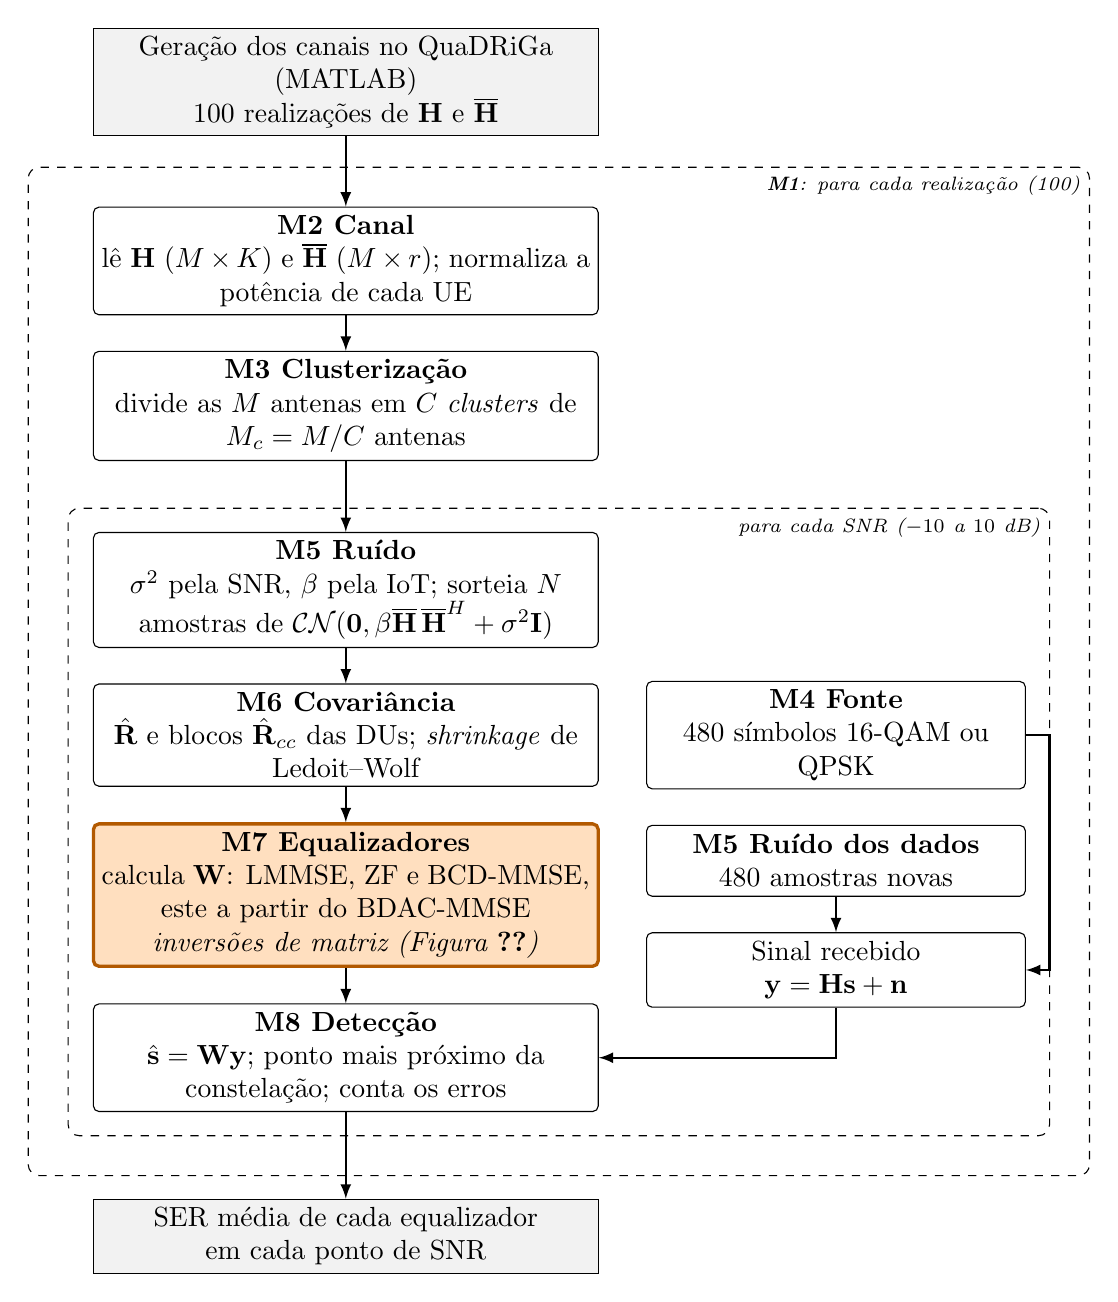
\begin{tikzpicture}[
    node distance = 0.45cm and 0.6cm,
    bloco/.style  = {draw, rounded corners=2pt, align=flush center, fill=white,
                     minimum height=0.9cm, text width=6.2cm, inner sep=3pt},
    lado/.style   = {draw, rounded corners=2pt, align=flush center, fill=white,
                     minimum height=0.9cm, text width=4.6cm, inner sep=3pt},
    dado/.style   = {draw, align=flush center, fill=gray!10,
                     minimum height=0.8cm, text width=6.2cm, inner sep=3pt},
    laco/.style   = {draw, dashed, rounded corners=4pt, inner sep=0.3cm},
    seta/.style   = {-latex, thick},
    inv/.style    = {fill=orange!25, draw=orange!70!black, very thick},
  ]

  % --- geração dos canais (MATLAB, uma vez) ---------------------------
  \node[dado] (quadriga) {Geração dos canais no QuaDRiGa (MATLAB)\\
    100 realizações de $\mathbf{H}$ e $\overline{\mathbf{H}}$};

  % --- laço das realizações -------------------------------------------
  \node[bloco, below=0.9cm of quadriga] (m2) {\textbf{M2 Canal}\\
    lê $\mathbf{H}$ ($M \times K$) e $\overline{\mathbf{H}}$ ($M \times r$);
    normaliza a potência de cada UE};
  \node[bloco, below=of m2] (m3) {\textbf{M3 Clusterização}\\
    divide as $M$ antenas em $C$ \textit{clusters} de $M_c = M/C$ antenas};

  % --- laço da SNR ------------------------------------------------------
  \node[bloco, below=0.9cm of m3] (m5) {\textbf{M5 Ruído}\\
    $\sigma^2$ pela SNR, $\beta$ pela IoT;
    sorteia $N$ amostras de $\mathcal{CN}(\mathbf{0}, \beta\overline{\mathbf{H}}\,\overline{\mathbf{H}}^H + \sigma^2\mathbf{I})$};
  \node[bloco, below=of m5] (m6) {\textbf{M6 Covariância}\\
    $\hat{\mathbf{R}}$ e blocos $\hat{\mathbf{R}}_{cc}$ das DUs;
    \textit{shrinkage} de Ledoit--Wolf};
  \node[bloco, inv, below=of m6] (m7) {\textbf{M7 Equalizadores}\\
    calcula $\mathbf{W}$: LMMSE, ZF e BCD-MMSE,\\
    este a partir do BDAC-MMSE\\
    \textit{inversões de matriz (Figura~\ref{fig:fluxo_m7})}};

  \node[lado, right=of m6] (m4) {\textbf{M4 Fonte}\\
    480 símbolos 16-QAM ou QPSK};
  \node[lado, below=of m4] (ruido) {\textbf{M5 Ruído dos dados}\\
    480 amostras novas};
  \node[lado, below=of ruido] (y) {Sinal recebido\\
    $\mathbf{y} = \mathbf{H}\mathbf{s} + \mathbf{n}$};

  \node[bloco, below=of m7] (m8) {\textbf{M8 Detecção}\\
    $\hat{\mathbf{s}} = \mathbf{W}\mathbf{y}$; ponto mais próximo
    da constelação; conta os erros};

  % --- saída ------------------------------------------------------------
  \node[dado, below=1.1cm of m8] (ser) {SER média de cada equalizador\\
    em cada ponto de SNR};

  % --- laços (M1) -------------------------------------------------------
  \begin{scope}[on background layer]
    \node[laco, fit=(m5) (m6) (m7) (m8) (m4) (ruido) (y)] (lacosnr) {};
    \node[laco, inner sep=0.5cm, fit=(m2) (m3) (lacosnr)] (lacoreal) {};
  \end{scope}
  \node[anchor=north east, font=\scriptsize\itshape]
    at (lacosnr.north east) {para cada SNR ($-10$ a $10$ dB)};
  \node[anchor=north east, font=\scriptsize\itshape]
    at (lacoreal.north east) {\textbf{M1}: para cada realização (100)};

  % --- setas ------------------------------------------------------------
  \draw[seta] (quadriga) -- (m2);
  \draw[seta] (m2) -- (m3);
  \draw[seta] (m3) -- (m5);
  \draw[seta] (m5) -- (m6);
  \draw[seta] (m6) -- (m7);
  \draw[seta] (m7) -- (m8);
  \draw[seta] (m4.east) -- ++(0.3,0) |- (y.east);
  \draw[seta] (ruido) -- (y);
  \draw[seta] (y) |- (m8);
  \draw[seta] (m8) -- (ser);
\end{tikzpicture}
\legend{Fonte: a autora.}
\end{figure}
